%%%%%%%%%%%%%%%%%%%%%%%%%%%%%%%%%%%%%%%%%%%%%%%%%%%%%%%%%%%%%%%%%%%%%%%%%%%%%%%
%%                                                           ENERGY CALIBRATION
%%%%%%%%%%%%%%%%%%%%%%%%%%%%%%%%%%%%%%%%%%%%%%%%%%%%%%%%%%%%%%%%%%%%%%%%%%%%%%%
%%                                          forward electron energy calibration 



%______________________________________________________________________________
%                                    Energiekalibration der Vorwärts-Elektronen
%
\chapter{Energiekalibration der Vorwärts-Elektronen}
\label{energy_calibration}

\begin{quote}
    Die Energiekalibration des elektromagnetischen Kalorimeters für Elektronen 
    ist von essentieller Bedeutung für Messung der Vorwärts-Rückwärts-
    Asymmetrie. Dieses Kapitel beschreibt die Kalibration für Elektronen mit
    hohen Pseudorapiditäten. Dabei wird zunächst auf \development 
\end{quote}



%______________________________________________________________________________
%                                                                    Grundlagen
%
\section{Grundlagen}
\label{energy_calibration:grundlagen}
\begin{itemize}
    \item Messung der Energie mit Kalorimeter (Verweis auf Detektor Kapitel)
    \item Notwendigkeit der Energiekalibration (Benötigte Präzision für 
        Vorwärts-Rückwärts-Asymmetrie)
    \item Vorangegangene Schritte ( Calibration-Hits, Test-Beam-Runs, 3-Stufen)
    \item Was im folgenden passiert (Vorwärts-Kalibration, in-situ
        kalibration, was ist noch zu kalibrieren)
    \item Zusätzliches Material
\end{itemize}



%______________________________________________________________________________
%                                                      Beschreibung der Methode 
%
\section{Beschreibung der Methode}
\label{energy_calibration:beschreibung_der_methode}

\begin{itemize}
    \item \sout{Betrachteter Prozess, CF-Ereignisse}
    \item Definition der Korrektur-Faktoren
    \item \sout{Annahmen (perfekte zentral-Elektronen)}
    \item Vereinfachung der Formeln und Extraktion
    \item 2-stufige Exktraktion
    \item Selektion und Samples
    \item Fit-Modelle, Effizienzkurve
\end{itemize}

Für die Kalibration der Vorwärts-Elektronen betrachtet man den elektroschwachen
Zerfalls-Prozess $Z/\gamma^* \rightarrow ee$ eines Z-Bosons in zwei
Elektronen\footnote{Die Bezeichnung \textit{Elektron} wird hier und im
Folgenden synonym für Elektronen und Positronen verwendet}. Dabei werden nur
Ereignisse selektiert, in denen eines der beiden Elektronen im Zentral-Bereich,
das andere im Vorwärts-Bereich detektiert wird. Diese Einbeziehung der Zentral-
Elektronen ist aus mehreren Gründen notwendig. Zum einen stehen entsprechende
Elektron-Trigger\footnote{siehe hierzu Kapitel
\ref{experimenteller_aufbau:atlas_detector:trigger-system}}
nur im Zentral-Bereich zur Verfügung. Zum anderen wäre die Selektion von
Ereignissen mit beiden Elektronen im Vorwärts-Bereich, in hohem Maße von
Untergrund-Prozessen dominiert, bei denen andere Objekte, überwiegend Jets,
fälschlicherweise als Elektronen rekonstruiert werden\footnote{vgl. Kapitel
\ref{experimenteller_aufbau:elektronen_in_atlas}}.
Allerdings stellt die Hinzunahme der Zentral-Elektronen die Kalibration der
Vorwärts-Elektronen ab initio in die Abhängigkeit einer vorangegangen 
Kalibration der Zentral-Elektronen.

Im folgenden Abschnitt werden zunächst einige grundlegende Annahmen eingeführt
und die Kalibration-Konstanten für Vorwärts-Elektronen definiert.


\subsection{Definitionen und Annahmen}
\label{energy_calibration:beschreibung_der_methode:definitionen_und_annahmen}

Die invariante Masse zweier relativistischer Teilchen, deren Ruhemassen
gegenüber ihren Energien vernachlässigt werden können, ergibt sich aus
\begin{equation}
    \label{invariant_mass:basic}
    m = \sqrt{ 2 \cdot E_1 E_2 (1-\cos\theta_{12}) }
\end{equation}
Dabei bezeichnet $E_{1/2}$ die Energie des Teilchens 1 bzw. 2 und $\theta_{12}$
den Öffnungswinkel zwischen beiden. Für die hier beschriebene Kalibration der
Vorwärts-Elektronen identifiziert man o.B.d.A. die Energie des Elektrons im
Zentral-Bereich mit $E_1$ und die Energie des Vorwärts-Elektrons mit $E_2$.

Man definiert nun den Kalibrations-Faktor $\alpha_i$, der die Abweichung zischen
wahrer und gemessener Energie korrigiert, wobei als beste Schätzung für die
\textit{wahre Energie} die \acs{MC}-Simulation des betrachteten Prozesses
herangezogen wird:
\begin{equation}
    \label{definition:energy_scale}
    E_\text{(data)} = E_\text{(MC)} (1+\alpha_i)
\end{equation}
Der Index $i$ weist darauf hin, dass für verschiedene Bereiche des
EM-Kalorimeters unterschiedliche Kalibrationskonstanten gelten. Man wählt eine
Unterteilung in der Pseudorapidität $\eta$, da mögliche Unterschiede vor allem
durch nicht-simuliertes passives Material, welches die Elektronen vor ihrem 
Eintritt in das Kalorimeter passieren, verursacht werden. Die grundsätzlich
inhomogene Verteilung von Materie vor dem Kalorimeter ist in Abbildung
\ref{fig:extra_material} dargestellt.
\begin{figure}
    \centering
    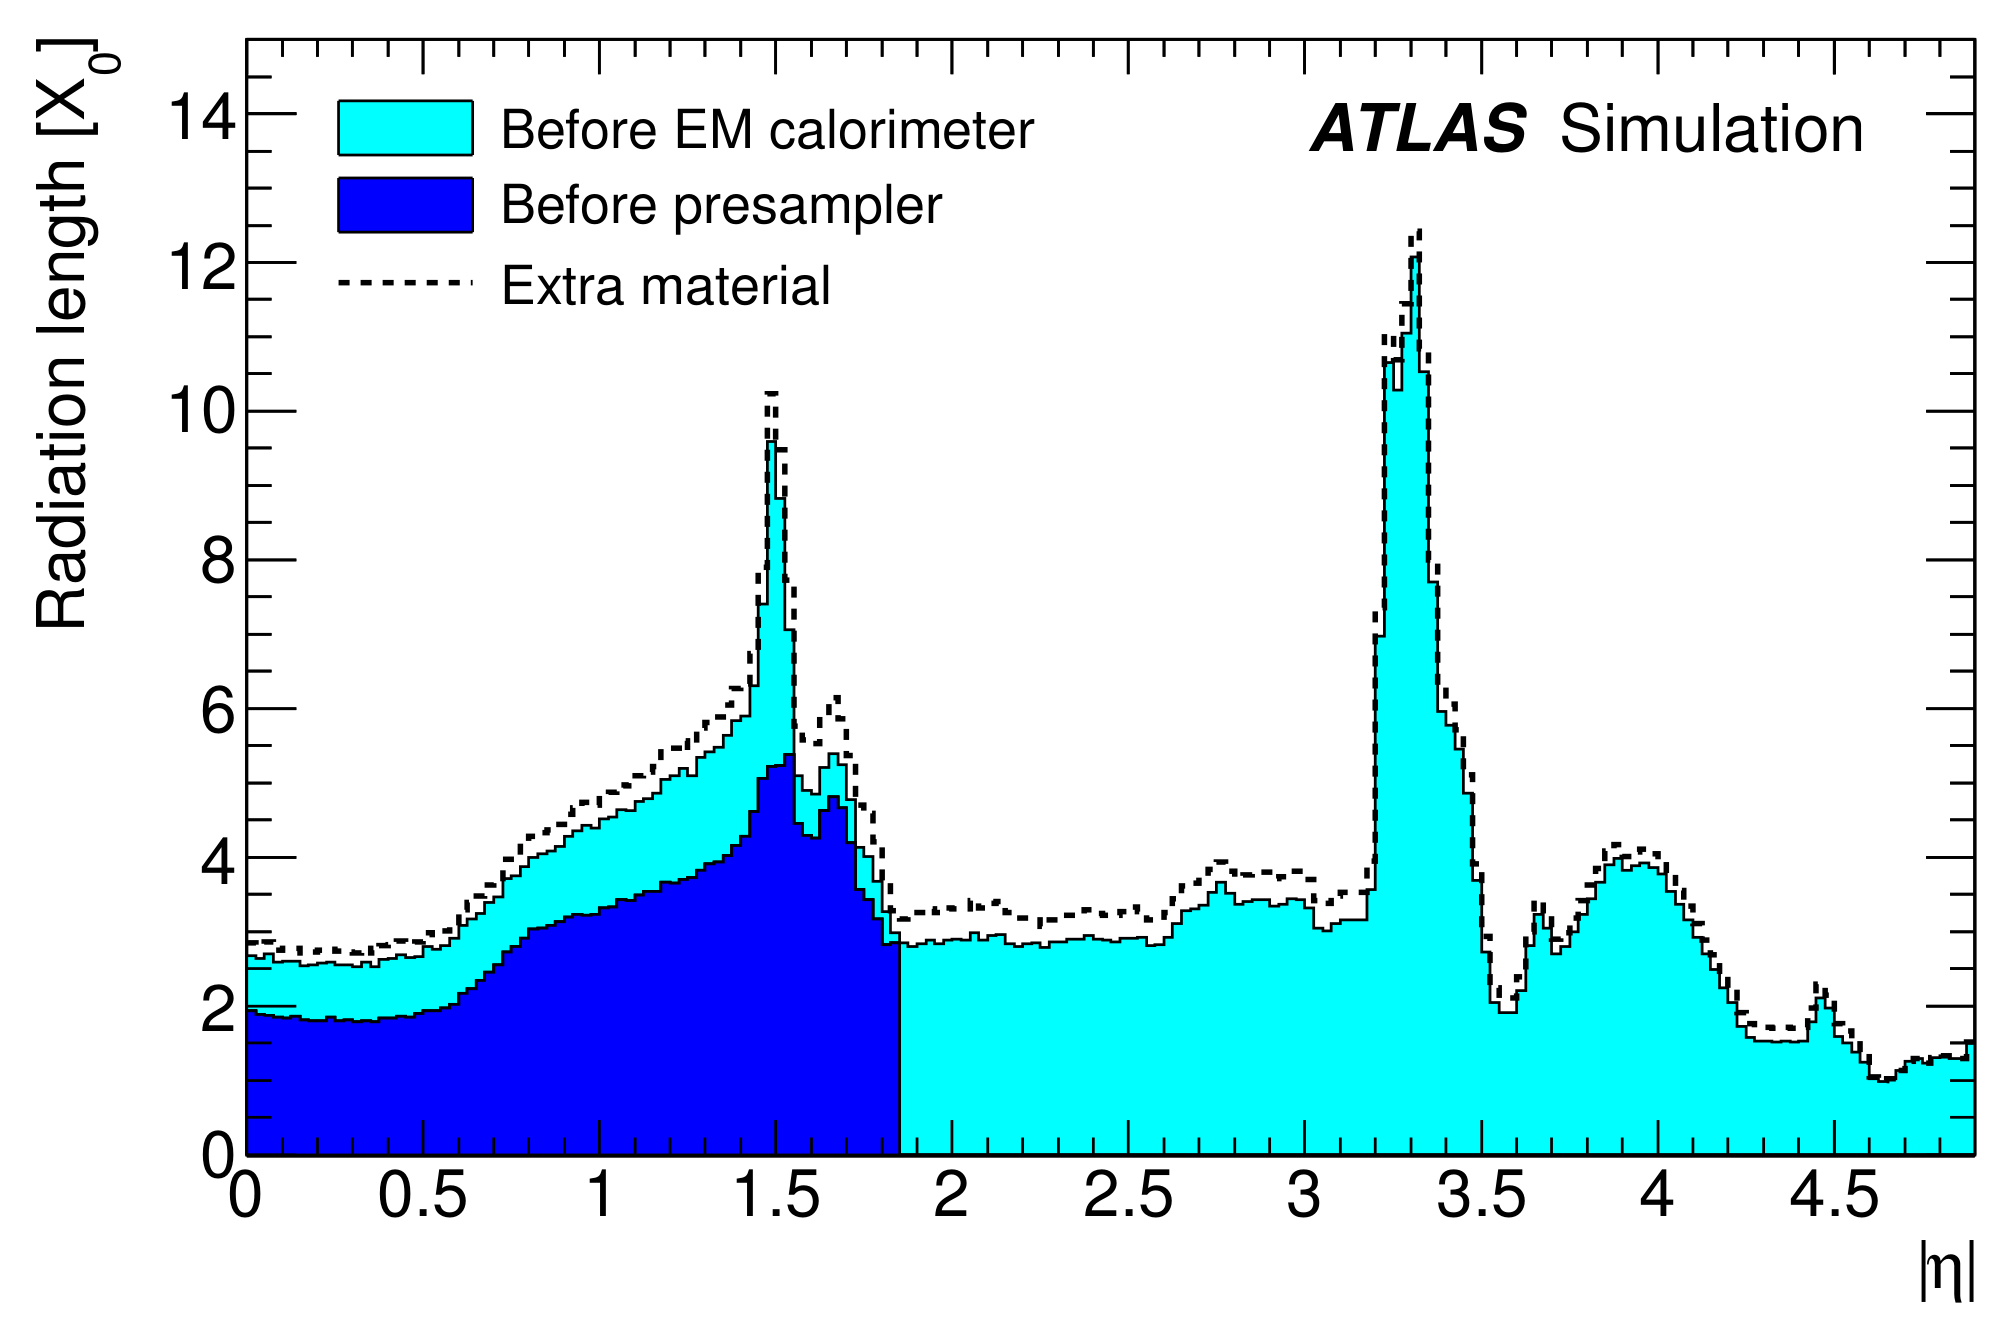
\includegraphics[width=0.7\textwidth]{img/extra_material}
    \caption[Material vor dem EM-Kalorimeter]
        {Die Menge an Material in Einheiten der Strahlungslänge $X_0$, die die
        Elektronen vor dem Kalorimeter durchfliegen, als Funktion der 
        Pseudorapidität $\eta$. Das zusätzliche Material wurde hier lediglich 
        zu systematischen Studien eingeführt und entspricht nicht der 
        tatsächlichen Verteilung. (Quelle: \cite{Aad:2011mk})}
    \label{fig:extra_material}
\end{figure}
Eine zusätzliche Unterteilung im Azimuthalwinkel $\phi$ wird nicht
vorgenommen, vielmehr geht man hier von einer isotropen Verteilung aus.

Wie bereits im einführenden Abschnitt \ref{energy_calibration:grundlagen}
erwähnt, werden die Elektronen im Zentral-Bereich als bereits perfekt
kalibriert angenommen, sodass gilt:
\begin{equation}
    \label{definition:perfect_central_electrons}
    E_\text{(data)}^\text{C} = E_\text{(MC)}^\text{C}
    \qquad \Longleftrightarrow \qquad
    \alpha_i^\text{C} = 0
    \qquad\qquad
    ^C : \text{zentral}
\end{equation}
Für die Messung der invarianten Masse (\ref{invariant_mass:basic}) des
\acs{CF}-Elektron-Paares folgt nun mit (\ref{definition:energy_scale}) und
(\ref{definition:perfect_central_electrons}):
\begin{align}
    m_\text{(data)}   &= \sqrt{ 2 \cdot E^C_\text{(data)} E^F_{\text{(data)}}
                         (1-\cos\theta)} 
                         \qquad ^C: \text{zentral}, \quad ^F: vorwärts
                         \nonumber \\[5pt]
                      &= \sqrt{ 2 \cdot E^C_\text{(MC)} E^F_{\text{(MC)}}
                         (1+\alpha^F_i)(1-\cos\theta)}
                         \nonumber \\[15pt]
    m^2_\text{(data)} &= 2 \cdot E^C_\text{(MC)} E^F_{\text{(MC)}}
                         (1+\alpha^F_i)(1-\cos\theta)
                         \nonumber \\[5pt]
                      &= m^2_\text{(MC)} (1+\alpha^F_i)
                         \label{eq:invariant_mass_sq}
\end{align}
Gleichung (\ref{eq:invariant_mass_sq}) liefert somit die Möglichkeit zur
Extraktion der Kalibrations-Faktoren $alpha_i^F$
\begin{equation}
    \label{eq:extraction_alpha}
    \alpha_i^F = \frac{m^2_\text{(data)}}{m^2_\text{(MC)}} - 1
\end{equation}
\development


%______________________________________________________________________________
%                                       Exktraktion der Kalibrations-Konstanten
%
\section{Extraktion der Kalibrations-Konstanten}
\label{energy_calibration:extraktion_der_kalibrations-konstanten}
\begin{itemize}
    \item Beispielhafte Fits
    \item Exktraktion der Energy-Scales
    \item Extraktion der Constant-Terms
    \item Systematiken
\end{itemize}



%______________________________________________________________________________
%                                                       Ergebnisse und Ausblick
%
\section{Ergebnisse und Ausblick}
\label{energy_calibration:ergebnisse_und_ausblick}
\begin{itemize}
    \item Zusammenfassung
    \item Diskussion ( Dominiert von Zentral-Skalen, Modell-Probleme )
    \item Verbesserungen ( Neue Zentral-Skalen, Template-Ansatz )
\end{itemize}


